\section{Diffusion/mean square displacement}
\todod{Diffusion normal to and parallel to surface?}
\todob{Plot of $r^2$ for 200 and 40 states to argue for origo move?}

% bulk diff in Ref \#1 = 0.202034846318
%   N = mean(47577, 47524, 47555, 47552, 47559) = 
% bulk diff in Ref \#2 = 0.178684448075
%   N = mean(50280, 50284, 50291, 50275, 50321)

% bulk diff in Rough \#1 = 0.197721045372      
%   N = mean(4271, 4279, 4252, 4294, 4284)
% bulk diff in Rough \#2 = 0.208658027239  
%   N = mean(3414, 3396, 3419, 3431, 3393)


We have measured the diffusion constant for water in the in all our systems, as function of distance to the silica matrix. We used 200 states for each system, with 100 timesteps of 0.050 picoseconds between each state (5 picoseconds between each state). To improve the statistics we divided each set of states into 5 non-overlapping origos, with 40 states per origo.\todoao{have we explained origo move anywhere?} The results are plotted in \crefrange{fig:first_diffusion_figure}{fig:last_diffusion_figure}. We have also measured the bulk diffusion constant, the results of which are listed in \cref{tab:bulk_water_diffusion}.

We first look at the diffusion as function of distance to the silica matrix in the four reference systems, which we have plotted in \cref{fig:diffusion_reference_systems}. We see that the diffusion constant, $D$, has similar quantitative behaviour as we move further from the silica matrix in all four reference systems, but that the actual $D$ is different in each system. The two systems with 86 \AA\ wide flat pores have diffusion constants that differ by around 10-30\%, even though those two systems should be pretty similar. The main difference between those two systems is the density, as we saw in \cref{sec:results_density}. We have listed the bulk $D$ in \cref{tab:bulk_water_diffusion}, and we see that the bulk diffusion for the two reference systems with 86 \AA\ wide flat pores is {0.202 \AA$^2$/ps}, while system \#2 has {0.179 \AA$^2$/ps}, with a difference of {13 \%}. \hl{So it seems like the increased density in reference system \#2 have had an impact on the diffusion -- so we use ref \#1 when comparing to other systems?}
%
%
% \begin{figure}[htpb]%
%     \centering%
%     \includesvg[width=0.6\textwidth, svgpath=./images/diffusion/]{diffusion_constant_move_origin_reference01}%
%     \caption{%
%         Diffusion constant as function of distance to silica matrix for all four reference systems (flat fractures). The solid lines are for the two systems with 86 \AA\ wide fractures, and the dashed lines for narrow fractures of 14.4 and 28.8 \AA. \hl{FINISH CAPTION}. %
%         \label{fig:diffusion_reference_systems}%
%     }%
% \end{figure}%

In \cref{fig:diffusion_rough_systems} we have plotted the diffusion constant %as function of distance from the silica matrix 
for the four random fracture systems, ``rough \#1'' through 4. We again see a quantitative similar behaviour, and we see that all systems except the 14.4 \AA\ narrow fracture (``rough \#3'') have very similar diffusion constants and behaviour. In \cref{tab:bulk_water_diffusion} see that the bulk diffusion constants in the two regular random fractures (\#1 and \#2) are similar, with a difference of {6 \%}. We also see that the $D$ for water at 7-10 \AA\ from the silica matrix is close to the bulk constant for these two systems.
\todoao{More about diffusion?}
%
% \begin{figure}[htpb]%
%     \centering%
%     \includesvg[width=0.6\textwidth, svgpath=./images/diffusion/]{diffusion_constant_move_origin_rough01}%
%     \caption{%
%         Diffusion constant as function of distance to silica matrix for all four random/rough fractures. \hl{FINISH CAPTION}. %
%         \label{fig:diffusion_rough_systems}%
%     }%
% \end{figure}%
%
%
% ---- Minipage ---- %
% \begin{figure}[htpb]%
% % \centering%
% \setlength{\myfigwidth}{0.58\textwidth}%
% \makebox[\textwidth][c]{ % to center figures below that are wider than \textwidth
%     \begin{minipage}[t]{\myfigwidth}%
%         \captionsetup{width=0.925\textwidth}%
%         \centering%
%         \includesvg[width=\textwidth, svgpath=./images/diffusion/]{diffusion_constant_move_origin_reference01}%
%         \caption{%
%             Diffusion constant ($D$) as function of distance to silica matrix ($r$) for all four reference systems (flat pores). The solid lines are the two systems with 86 \AA\ wide pores, and the dashed lines are 14.4 and 28.8 \AA\ narrow flat pores. \hl{FINISH CAPTION}. %
%             \label{fig:diffusion_reference_systems}%
%         }%
%     \end{minipage}%
%     \hfill%
%     \begin{minipage}[t]{\myfigwidth}% % change "b" to "t" to anchor top instead of bottom
%         \captionsetup{width=0.925\textwidth}% % minipage defines a \textwidth for it's own, so we have to repeat this command inside the minipage
%         \centering%
%         \includesvg[width=\textwidth, svgpath=./images/diffusion/]{diffusion_constant_move_origin_rough01}%
%         \caption{%
%             Diffusion constant ($D$) as function of distance to silica matrix ($r$) for all four random rough fractures. Solid lines are regular random fractures, and dashed lines are narrow fractures with uniform width of 14.4 and 28.8 \AA. \hl{FINISH CAPTION}. %
%             \label{fig:diffusion_rough_systems}%
%         }%
%     \end{minipage}%
% }
% \end{figure}%
%
% ---- Subcaption ---- %
\begin{figure}[htpb]%
% \centering%
\setlength{\myfigwidth}{0.58\textwidth}%
\makebox[\textwidth][c]{ % to center figures below that are wider than \textwidth
    \begin{minipage}[t]{\myfigwidth}%
        \centering%
        \includesvg[width=\textwidth, svgpath=./images/diffusion/]{diffusion_constant_move_origin_reference01}%
        \subcaption{\label{fig:diffusion_reference_systems}}%
    \end{minipage}%
    \hfill%
    \begin{minipage}[t]{\myfigwidth}% % change "b" to "t" to anchor top instead of bottom
        \centering%
        \includesvg[width=\textwidth, svgpath=./images/diffusion/]{diffusion_constant_move_origin_rough01}%
        \subcaption{\label{fig:diffusion_rough_systems}}%
    \end{minipage}%
}%
\caption{%
    Diffusion constant ($D$) as function of distance from silica matrix ($r$), for \textbf{a)} all reference systems and \textbf{b)} all rough fractures. Dashed lines are 14.4 and 28.8 \AA\ \textbf{a)} flat pores and \textbf{b)} narrow, uniform width fractures. \hl{FINISH CAPTION}. %
    \label{fig:first_diffusion_figure}%
}%
\end{figure}%

% \begin{figure}[htpb]%
%     \centering%
%     {
%         \newcommand{\f}{\footnotesize}
%         \includesvg[width=0.7\textwidth, svgpath=./images/diffusion/]{diffusion01}%
%     }
%     \caption{%
%         Diffusion. \hl{Make new figure using new diffusion program}. %
% %         \label{fig:cell_lists}%
%     }%
% \end{figure}%

% \begin{figure}[htpb]%
%     \centering%
%     {
%         \newcommand{\f}{\footnotesize}%
%         \includesvg[width=0.7\textwidth, svgpath=./images/diffusion/]{diffusion_constant02}%
%     }
%     \caption{%
%         Diffusion. \hl{Make new figure using new diffusion program} \hl{FINISH CAPTION}. %
% %         \label{fig:cell_lists}%
%     }%
% \end{figure}%

The bulk diffusion constants have been estimated in the two reference systems with 86 \AA\ wide flat pores (reference \#1 and \#2), and in rough system \#1 and \#2, by measuring $D$ for all water molecules further away from the silica matrix than 10 \AA. The results can be seen in \cref{tab:bulk_water_diffusion}. The other four systems have very narrow pores and fractures, with most of the water molecules closer to the silica matrix than 10 \AA\, so we haven't measured the bulk diffusion in those systems, and we don't expect much of the water to have bulk behaviour\todobo{explain this better?}.
%
\begin{table}[!htb]%
    \centering%
    \begin{tabular}{l|cc}%
        \textit{System} & Bulk $D$ [\AA$^2$/ps] & N    \\\hline
        Reference \#1   & 0.202                 & 48k  \\ % 0.202034846318
        Reference \#2   & 0.179                 & 50k  \\ % 0.178684448075
        Rough \#1       & 0.198                 & 4.3k \\ % 0.197721045372
        Rough \#2       & 0.209                 & 3.4k \\ % 0.208658027239
    \end{tabular}%
    \vspace{8pt}%
    \caption{%
        Bulk diffusion constant for water (for $r>10$ \AA), and the number of water molecules used in the calculations. %
        \label{tab:bulk_water_diffusion}%
    }%
\end{table}

In \cref{fig:diffusion_normal_and_reference} we have plotted diffusion for the two normal random fractures (with varying pore width) together with all four reference systems. We see that the behaviour of $D$ as function of the distance to the silica matrix in the two fracture systems is very similar to each other, and matches the behaviour in reference system \#1 pretty well. This reference system is the one with a 86 \AA\ wide flat pore and the lowest bulk density of the two reference systems with wide flat pores ($\rho \approx 1038$ kg/m$^3$ compared to $\approx 1091$ kg/m$^3$).
\todoa{Write something about rough vs. reference and uniform rough vs. narrow flat pore figures below.}%

In \cref{fig:diffusion_narrow_and_reference} we have plotted the diffusion for the two random narrow fractures with uniform width together with all four reference systems. We see that the diffusion in the 14.4 \AA\ narrow fracture (``Rough \#3'') almost exactly matches the the diffusion in the reference system with a 14.4 \AA\ flat pore (``Ref \#4''). We also see that the 28.8 \AA\ narrow fracture (``Rough \#4'') has higher diffusion than the flat reference system with a 28.8 \AA\ flat pore (``Ref \#4''), but that it matches the reference system with a 86 \AA\ flat pore (``Ref \#1'') very well\todobo{discuss this?}.
%
% ---- Minipage version ---- %
% \begin{figure}[htpb]%
% % \centering%
% \setlength{\myfigwidth}{0.58\textwidth}%
% \makebox[\textwidth][c]{ % to center figures below that are wider than \textwidth
%     \begin{minipage}[t]{\myfigwidth}%
%         \captionsetup{width=0.925\textwidth}%
%         \centering%
%         \includesvg[width=\textwidth, svgpath=./images/diffusion/]{diffusion_constant_move_origin_normal01}%
%         \caption{%
%             Diffusion constant ($D$) as function of distance from silica matrix ($r$), for random rough fractures and all reference systems. \hl{reference figure or remove} \hl{FINISH CAPTION}. %
%             \label{fig:diffusion_normal_and_reference}%
%         }%
%     \end{minipage}%
%     \hfill%
%     \begin{minipage}[t]{\myfigwidth}% % change "b" to "t" to anchor top instead of bottom
%         \captionsetup{width=0.925\textwidth}% % minipage defines a \textwidth for it's own, so we have to repeat this command inside the minipage
%         \centering%
%         \includesvg[width=\textwidth, svgpath=./images/diffusion/]{diffusion_constant_move_origin_narrow01}%
%         \caption{%
%             Diffusion constant ($D$) as function of distance from silica matrix ($r$), for random narrow fractures and all reference systems. \hl{reference figure or remove} \hl{FINISH CAPTION}. %
%             \label{fig:diffusion_narrow_and_reference}%
%         }%
%     \end{minipage}%
% }
% \end{figure}%
%
% ---- Subcaption/subfigure version ---- %
\begin{figure}[htpb]%
% \centering%
\setlength{\myfigwidth}{0.58\textwidth}%
\makebox[\textwidth][c]{ % to center figures below that are wider than \textwidth
    \begin{minipage}[t]{\myfigwidth}%
        \centering%
        \includesvg[width=\textwidth, svgpath=./images/diffusion/]{diffusion_constant_move_origin_normal01}%
        \subcaption{\label{fig:diffusion_normal_and_reference}}%
    \end{minipage}%
    \hfill%
    \begin{minipage}[t]{\myfigwidth}% % change "b" to "t" to anchor top instead of bottom
        \centering%
        \includesvg[width=\textwidth, svgpath=./images/diffusion/]{diffusion_constant_move_origin_narrow01}%
        \subcaption{\label{fig:diffusion_narrow_and_reference}}%
    \end{minipage}%
}%
\caption{%
    Diffusion constant ($D$) as function of distance from silica matrix ($r$), for \textbf{a)} rough fracture system \#1 and \#2 (normal rough fractures) and all reference systems, and \textbf{b)} the narrow uniform width fractures (fracture system \#3 and \#4) and all reference systems. Dashed lines are reference systems. %
    \label{fig:last_diffusion_figure}%
}%
\end{figure}%

% \begin{figure}[htpb]%
%     \centering%
%     \includesvg[width=0.8\textwidth, svgpath=./images/diffusion/]{diffusion_constant_move_origin_normal01}%
%     \caption{%
%         Diffusion for random rough fractures and reference systems. \hl{reference figure or remove} \hl{FINISH CAPTION}. %
% %         \label{fig:cell_lists}%
%     }%
% \end{figure}%
% 
% \begin{figure}[htpb]%
%     \centering%
%     \includesvg[width=0.8\textwidth, svgpath=./images/diffusion/]{diffusion_constant_move_origin_narrow01}%
%     \caption{%
%         Diffusion for random narrow fractures and reference systems. \hl{reference figure or remove} \hl{FINISH CAPTION}. %
% %         \label{fig:cell_lists}%
%     }%
% \end{figure}%

% \begin{figure}[htpb]%
%     \centering%
%     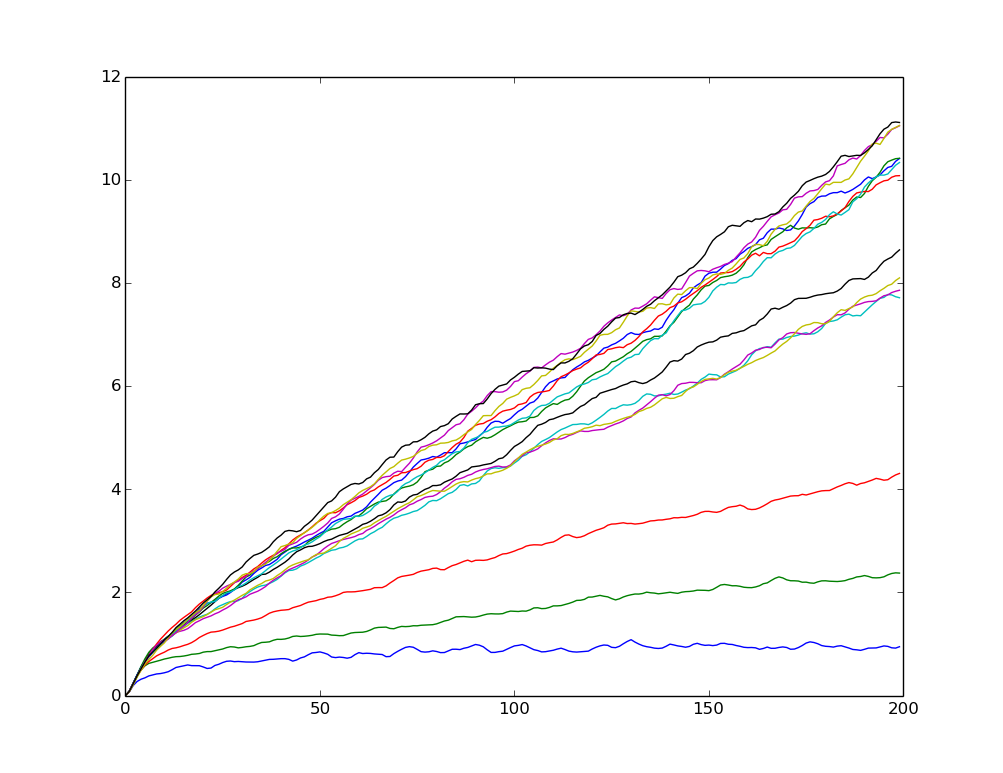
\includegraphics[width=0.5\textwidth]{images/diffusion/mean_square_displacement_interesting.png}%
%     \caption{%
%         Something interesting (msd stops increasing for a couple of angstrom near 4.5-5, 5-5.5, 5.5-6.0) \hl{reference figure or remove} \hl{FINISH CAPTION}. %
% %         \label{fig:cell_lists}%
%     }%
% \end{figure}%

% \begin{figure}[htpb]%
%     \centering%
%     \setlength{\myfigwidth}{0.49\textwidth}%
% %     \setlength{\mycaptionwidth}{0.3\textwidth}%
% %
%     \begin{subfigure}[b]{\myfigwidth}%
%         \includesvg[width=\textwidth, svgpath=./images/diffusion/]{diffusion_constant_move_origin01}%
%         \caption{%
%             Diffusion. \hl{FINISH CAPTION}. %
%     %         \label{fig:cell_lists}%
%         }%
%     \end{subfigure}%
%     \hfill%
%     \begin{subfigure}[b]{\myfigwidth}%
%         \includesvg[width=\textwidth, svgpath=./images/diffusion/]{diffusion_constant_move_origin02}%
%         \caption{%
%             Diffusion. \hl{FINISH CAPTION}. %
%     %         \label{fig:cell_lists}%
%         }%
%     \end{subfigure}%
%     \caption{%
%         rough\_fracture\_01\_abel - ``Rough fracture \#1'' \hl{Caption} %
%         \label{fig:renderings_rough_fracture01_abel}%
%     }%
% \end{figure}%